

\section{Evaluation}
\label{sec:evaluation}

We plan to evaluate our method in two ways. Primarily, the methods ability to handle failure. To cope with the failure gracefully and cause the least amount of disturbance in the gameplay as possible. A secondary goal is to keep the latency of the game down as more clients and server are added to the system.

\subsection{Fault Tolerance}

The goal of the system was to gracefully cope with failing nodes without introducing latency. 
A game system design may choose to pause the processing of the game until the \gamestate becomes consistent again, during this time the players must wait for the game state to synchronize.
Game flow and minimal latency (\todo{as seen from a player of the game}) is prioritized for consistency for this project.
In order to reduce latency consistency is sacrificed. 
When a node fails it could take a short amount of time to detect this failure as an inactivity.
During this time the agent for that node still exists in the game but is immobile.

Overall the system works as desired for graceful fault tolerance.
When a node fails the agent exists in the \gamestate for every node for a short period of time (a few seconds) after which all data related to the agent is removed from the \gamestate.

\subsection{Scalability vs Consistency}

It is difficult to measure the consistency between each of the nodes. 
We would have to employ a large logging system that would take snap shots of the \gamestate at points in time. 
In order for these snapshots to be effective there would need to be additional time synchronization across the nodes for comparison. 
Instead the relative number of successful shots is used to measure consistency. 
A successful shot is one that is initiated by a client, forwarded to the client's local server and again forwarded to the proper server for validation. 
The shot is successful if the last server agrees with the result of the shot. 
The occurrence of successful shot implies that $3$ \gamestates where at least partial consistent.
We measure the scalability by increasing the number of nodes in the system and comparing the relative number of fire events that are successful. 

	\begin{figure}[ht]
	\centering
		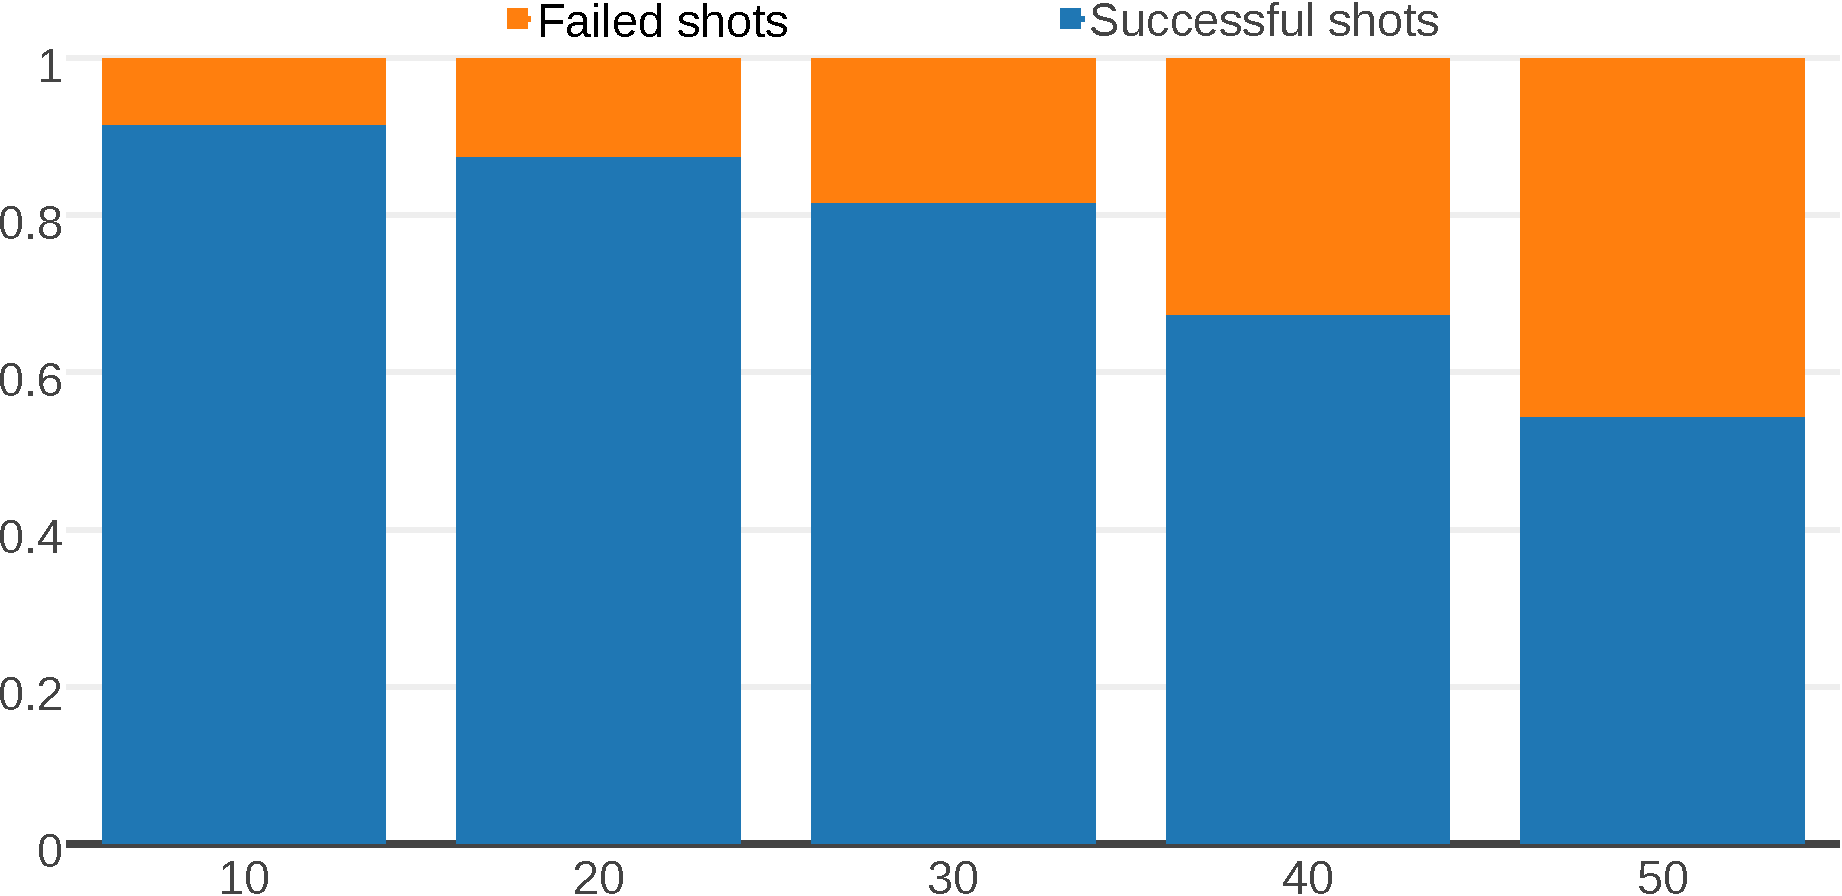
\includegraphics[width=0.95\linewidth]{../images/agents-vs-consistency-via-shots-crop.pdf}
		agents
		\caption{\label{figure:nodes-vs-shots-consistency} A chart of the relative numbers of successful shots vs failed shots. As the number of nodes in the system increases the relative number of successful shots decreases.}
	\end{figure}
Figure~\ref{figure:nodes-vs-shots-consistency} shows us how well the systems consistency copes with the number of nodes in the system. As expected, as the number of nodes increases the number of successful shots decreases. The decrease in successful shots is a proxy for the system consistency. 
This is the result of increased latency and dropped packets in the system. 

\subsection{Game Visualization}

\begin{figure}[htb]
\centering
	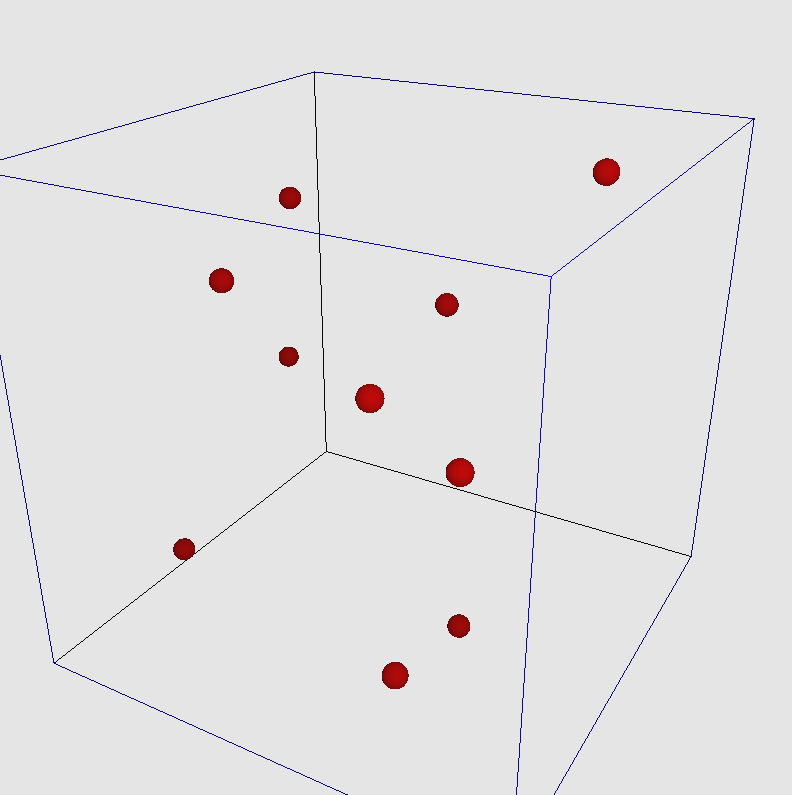
\includegraphics[width=0.45\linewidth]{../images/10-agents-render.png}
	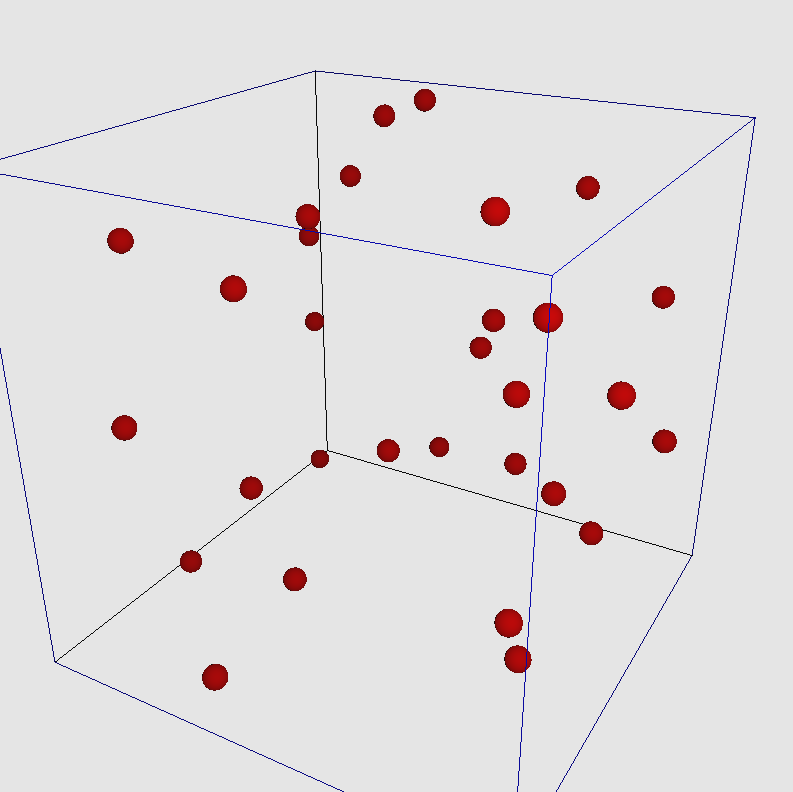
\includegraphics[width=0.45\linewidth]{../images/30-agents-render.png}	

	\caption{\label{figure:game-renders} Two rasterized simulation frames. On the left with $10$ agents and on the right with $30$ agents.}
\end{figure}